% !TEX root = ../Lazcorreta.Tesis.tex
% !TEX root = ../../Lazcorreta.Tesis.tex
\ABIERTO
%Los trabajos expuestos en los capítulos anteriores muestran una dificultad presente en muchas investigaciones en el ámbito de la informática, la imposibilidad de comprobar si los resultados obtenidos son correctos y aplicables con la tecnología actual. Todas las Ciencias recogen una Teoría que la sustenta, la Informática también, pero las demostraciones teóricas basadas en otras Ciencias no siempre son válidas para la Informática. Hay muchos artículos teóricos sobre Minería de Datos, pero algunos de ellos no evolucionan en un artículo posterior que muestre cómo se ha realizado el experimento con la tecnología actual usando datos reales.
%
%Es fácil calcular teóricamente el número de reglas de asociación presente en una colección concreta de datos, pero si el algoritmo propuesto no es capaz de almacenar en RAM todas las reglas de asociación del problema no servirá de nada ese algoritmo en esa situación. \texttt{mushroom} fue el primer caso que encontré curioso en el ambicioso campo de la Minería de Datos, una colección de tan solo 5\,644 registros de 23 valores que sólo contenía 100 valores diferentes no podía ser analizada a fondo por el mejor algoritmo de ARM que conozco, Apriori, cuando el número de transacciones distintas que se puede obtener bajo estas circunstancias es X\,XXX\,XXX y con ellas tenemos un máximo de X\,XXX\,XXX\,XXX\,XXX reglas de asociación. La tecnología actual de un equipo de escritorio no puede gestionar en RAM tanta información, pero me negaba a creer que no se pudiera extraer \emph{toda la información} que contuviera un problema tan pequeño. Al profundizar en \texttt{mushroom} y los artículos que lo mencionaban y otras colecciones de datos que encontré publicadas en los mismos portales encontré un modo de indicar al algoritmo de ARM que estoy tratando con un tipo de colecciones de datos especial. No es simplemente una colección de transacciones como las analizadas en~\ref{sec:arm:conceptos-basicos} si no que éstas tienen unas restricciones muy fuertes en su definición.
%
%Este informe refleja el trabajo que he realizado para descubrir lo suficiente como para ser merecedor del título de doctor en Informática. Los anteriores capítulos reflejan una gran labor de documentación y exposición científica de los resultados que podía obtener con colecciones de datos fijas, no disponía de un servidor capaz de poner a prueba nuestras aportaciones y realizar sugerencias en tiempo real a un gran número de usuarios. Podía comprobar que mis cálculos se podían realizar con la tecnología actual y las colecciones de datos que yo manejaba pero no sabía qué ocurriría si aumentaran mis colecciones de datos o si pudiera realizar sugerencias en tiempo real. Es un buen trabajo teórico apoyado en algunas realizaciones prácticas pero del que no puedo extraer aún la conclusión que es un buen trabajo de investigación en Informática.

%TODO: Buscar la cita de gAcademy o eliminar
Uno de los problemas de la búsqueda de \ars mediante equipos informáticos es su necesidad de memoria RAM para guardar todos los \itemsets frecuentes (\aprioriL) en un lugar de rápido acceso para ser más eficientes en la búsqueda de \ars. El \dilemaIR puede aparecer en cualquier momento, dependiendo de los datos que contenga el almacén \D que estemos analizando, y se siguen proponiendo ideas para aliviarlo como el uso de umbrales automáticos para el \soporte propuesto por~\citet{SadhasivamAngamuthu-MiningRareItemsetWithAutomatedSupportThresholds-2011}. Sería interesante poder averiguar, en base a información básica del fichero \D, qué requisitos de memoria RAM necesitamos, de cuáles disponemos y, con ello, deducir hasta qué \soporte mínimo podemos trabajar con esa colección específica de datos en este equipo en particular \citep{JinMcCallenBreitbartFuhryWang-EstimatingTheNumberOfFIInLargeDB-2009,Lhote-NumberOfFPInRandomDBs-2009}. Aunque este proceso puede llevar algo de tiempo y restar eficiencia global al algoritmo de \FIM permite ahorrar el tiempo perdido cuando el programa deja de funcionar por falta de RAM y no es capaz de ofrecernos ningún resultado.

%TODO: Reorganizar, algo de esto se menta en el primer párrafo
%TODO: Ojo, el enlace queda en un salto de página y afecta a la cabecera de la siguiente página. COMPROBARLO EN LA VERSIÓN FINAL
Esta reflexión tiene sentido si pensamos en grandes \datasets pero nos llamó la atención en ficheros tan "`pequeños"' como \texttt{chess.dat} o \mushroom. \mushroom es una colección de datos ampliamente utilizada debido a su publicación en \urlConNotaAlPie{https://archive.ics.uci.edu/ml/datasets/Mushroom}{UCI - Machine Learning Repository}, donde podemos encontrar una completa descripción de los datos en sí y de su aparición en el mundo de la investigación. Encontramos información sobre el uso de este almacén \D en artículos de \clasificacion.

%TODO: Añadir ZakiPetersAssentSeidl_Clicks_06 y Ziani:Ouinten:MiningMaximalFIJavaImplOfFPMAXalgorithm:09 (dea.bib) 
Estos ficheros han sido analizados en muchos artículos desde el punto de vista de la \arm clásica~\citep{Suzuki-DiscoveringInterestingExceptionRulesWithRulePair-2004, Borgelt-EfficientImplementationsOfAprioriAndEclat-2004, ThabtahCowlingHammoud-ImprovingRuleSorting-2006, WangXinCoenen-MiningEfficientlySignificantCAR-2008, LiZhang-MiningMaximalFIOnGraphicsProcessors-2010, MalikRaheja-ImprovingPerformanceOfFrequentItemsetAlgorithm-2013, RituArora-IntensificationOfExecutionOfFrequentItemSetAlgorithms-2014, SahooKumarGoswami-AnAlgorithmForMiningHighUtilityClosedItemsetsAndGenerators-2014}. Se proponen nuevas medidas, como la \emph{utilidad} de los \itemsets~\citep{WuShie-MiningTopKHighUtilityItemsets-2012} para aliviar el \dilemaIR. En todos los casos se ha de recurrir al \soporte mínimo para poder llevar a cabo el análisis en un tiempo prudencial (algo más de 2 segundos en el caso de~\citeauthor{RituArora-IntensificationOfExecutionOfFrequentItemSetAlgorithms-2014}, un estudio muy reciente cuyos gráficos coinciden con los de~\citeauthor{MalikRaheja-ImprovingPerformanceOfFrequentItemsetAlgorithm-2013}). Intentamos aplicar técnicas de \dm a colecciones relativamente pequeñas (\mushroom sólo contiene $8\,124 \times 23$ datos combinando 119 ítems distintos) y no podemos profundizar o trabajar en tiempo real si no aplicamos recortes drásticos de información. Hoy en día, almacenes \D de este tamaño deberían poder analizarse en tiempos razonables sin prescindir de ninguno de sus datos.

Antes de obtener más información sobre \mushroom comenzamos a analizar los resultados obtenidos en nuestros propios experimentos sobre este almacén \D. Al observarlos encontramos una estructura concreta: todas las filas ("`\transacciones"') tienen el mismo número de datos y en la primera columna sólo aparece un 1 o un 2, en la segunda sólo un 3, 4 o 5\ldots Se trata de una estructura muy rígida y con exceso de información. Al descubrir que el 1 aparecía en 3\,916 \transacciones dedujimos y comprobamos que el 2 aparecería en las restantes 8\,124 - 3\,916 . En el proceso de \fim estábamos desperdiciando esta información y nos entreteníamos en contar el número de veces que aparecía el ítem 2. También descubrimos que el ítem 3 aparecía en un total de 3\,656 \transacciones, en 1\,708 ocasiones junto al ítem 1, luego en las restantes 3\,656 - 1\,708 veces que aparece ha de estar junto al ítem 2. No necesitamos averiguar nada sobre el ítem 2, lo que averigüemos sobre el ítem 1 y la información estructural del \dataset nos dará toda la información que tiene \D sobre el ítem 2. No necesitamos utilizar memoria RAM para guardar información sobre el ítem 2, tendremos memoria RAM libre para analizar los \irs más frecuentes de \D o incluso para obtener información sobre todos los ítems en estudio.

Nuestros primeros análisis sobre \mushroom cumplieron con nuestras expectativas, tras la primera lectura de \D podíamos comprobar que las \transacciones tenían una estructura que podía ser utilizada para ahorrar recursos de memoria y obtuvimos \emph{todas} las \ARs que tiene el fichero sin tener que recurrir al uso de \soporte mínimo, todo ello en pocos segundos y con un consumo de RAM aceptable para cualquier equipo de sobremesa.

%TODO: Revisar esta información
\borrar{Mejorar}La Minería de Reglas de \Clasificacion (CRM) toma pronto las bondades de la Minería de Reglas de Asociación (ARM) derivando en una nueva línea de investigación en auge denominada \carm (\CARM) ~\citep{LiuHsuMa-IntegratingClassificationAndARM-1998, Bayardo-EfficientlyMiningLongPatternsFromDB-1998, WangXinCoenen-MiningEfficientlySignificantCAR-2008} donde se aprovecha el potencial que tienen las \ars para descubrir clasificadores precisos. CARM transforma los \datasets que han de ser analizados desde la perspectiva de CRM para que puedan ser vistos como conjuntos de transacciones y hacer un análisis basado en ARM. Para ello convierten los valores utilizados en CRM, formado por pares atributo=valor, en atributos binarios que tendrán el significado "`Si aparece el atributo binario X entonces el registro toma el valor Y en el atributo original $\A_i$"'. Ha habido grandes avances en \Clasificacion gracias a esta pequeña transformación, sin embargo también se ha perdido información muy importante sobre el \dataset en estudio, que no será aprovechada si no la incorporamos a la colección de transacciones que queremos analizar con ARM.

Tras llevar a cabo la investigación que se expone en este capítulo podemos afirmar que, aunque muchas de las citas revisadas han experimentado con \mushroom para aliviar su \dilemaIR, \mushroom y muchos \datasets de similares características realmente no contienen \IRs y contienen información redundante que puede ser ignorada para trabajar con más profundidad sobre el problema de \Clasificacion para el que han sido creados. 

Por último, introducimos y modelizamos los conceptos de \Catalogo y \CC con los que se puede analizar de forma más eficiente la información contenida estos ficheros y mejorar el proceso de \Clasificacion en muchos de los problemas ya estudiados y en todos aquellos que se puedan plantear en el futuro siguiendo las pautas marcadas en esta investgación. 





\section{Transacciones Estructuradas}
\label{sec:clasificacion:transacciones-tipo-ii}
% !TEX root = ../../Lazcorreta.Tesis.tex
% !TEX root = ../../../Lazcorreta.Tesis.tex
%\ABIERTO
Desde sus inicios la \ARM se ha protegido del \dilemaIR mediante la definición de un \soporte mínimo que impide estudiar los ítems de menor soporte (\irs) para evitar problemas de desbordamiento de memoria y poder ofrecer resultados en poco tiempo. En la evolución del \ARM hay múltiples aportaciones que alivian este problema pero siempre a costa de renunciar al estudio de algunas relaciones existentes entre los datos en estudio.

En los primeros trabajos sobre \ARM se trataba de evitar la búsqueda de relaciones entre los \irs \citep{AgrawalImielinskiSwami-MiningAssociationRulesBetweenSetsOfItemsInLargeDB-1993,AgrawalSrikant-FastAlgorithmsForMiningAssociationRules-1994,ParkChenYu-UsingAHashBasedMethod-1997}. En \cite{LiuHsuMa-ARMWithMultipleMS-1999}, proponen el uso de múltiples soportes mínimos para que un \itemset sea considerado frecuente sólo si su \soporte es grande en relación al \soporte de los ítems que lo forman. De este modo se ahorra espacio en memoria que puede ser utilizado para analizar ítems con menor \soporte. El uso de un \soporte relativo para cada \itemset basado en la \confianza de las \ars que generan sus ítems, lo que permite guardar información de los \itemsets con menor \soporte que el \soporte mínimo que superen su \soporte relativo \citep{YunHaHwangRyu-MiningAROnSignificantRareDataUsingRelativeSupport-2003}, garantizando que las reglas que generan sean de calidad. En \cite{HuChen-MiningARwithMMS-2006}, se propone una mejora del algoritmo propuesto en \cite{LiuHsuMa-ARMWithMultipleMS-1999}, para dotarlo de escalabilidad. En \cite{TsengLin-EfficientMiningOfAR-2007}, trabajan con las mismas ideas de \soporte múltiple pero reducen el número de \itemsets a guardar en función de su \lift, que mide la mejora que produce la presencia de un ítem en el soporte del resto de ítems que contiene. En \cite{KiranReddy-ImprovedMultipleMSBasedAppMineRareAR-2009}, utilizan múltiples \soportes basados en la distribución conjunta de los ítems y no sólo en su distribución individual como proponían en \cite{LiuHsuMa-ARMWithMultipleMS-1999}. Todas estas aportaciones reducen el número de itemsets almacenados en memoria, con lo que pueden almacenarse otros \itemsets menos frecuentes pero con mejor información sobre la población en estudio.

Cuando trabajamos con un número grande de ítems diferentes y una gran cantidad de \transacciones el \dilemaIR sólo es resoluble utilizando mucho tiempo y/o potentes computadores. Lo que sorprende es que este dilema aparezca en colecciones de datos con dimensiones reducidas, como ocurre con muchos repositorios utilizados en artículos sobre el problema de \Clasificacion que incorporan técnicas de \arm.

Es el caso de \texttt{chess.dat} y \mushroom.  \texttt{chess} recoge información sobre la posición final de una serie de piezas en el juego del ajedrez, contiene tan solo 75 ítems distintos en un total de 3\,196 transacciones. \texttt{mushroom} recoge el valor de una serie de atributos medidos en ciertas setas, utilizando 119 ítems distintos en 8\,124 transacciones. Todos los investigadores que han trabajado con estas colecciones han tratado sus transacciones del mismo modo que la clásica \transaccion formada por la ``cesta de la compra''. En esta sección mostramos que se puede dar un tratamiento diferente sin perder las ventajas del \ARM ni aplicar nuevos algoritmos.





\subsection{Tipos de \transacciones}
\label{sec:clasificacion:transacciones-tipo-ii:tipos-de-transacciones}
% !TEX root = ../../../Lazcorreta.Tesis.tex
\ABIERTO
La definición de \transaccion (véase pg.~\pageref{def:1:3:2:transaccion}) es muy elemental: ``conjunto de ítems observados en ciertas circunstancias''. Esta simple definición permite modelar muchas colecciones de datos mediante \transacciones, desde la clásica ``cesta de la compra'' hasta el estudio de una \sn web -- como si se tratara de un conjunto de páginas web visitadas conjuntamente -- pasando por la observación de las características de individuos que tienen enfermedades similares o la detección de fraude en el uso de tarjetas de crédito. En este capítulo estamos trabajando con la observación de ciertas características de los individuos de una población, ejemplarizando en el fichero \mushroom.

Si suponemos que no es casual el hecho de formar una \transaccion agrupando unos ítems y no otros, y observamos un conjunto grande de \transacciones, no es difícil pensar que encontraremos en ellas conjuntos de ítems que se repiten, a los que llamamos \itemsets frecuentes o patrones. Por ejemplo, en la cesta de la compra estos patrones nos pueden sugerir que ``el cliente que compra el producto $A$ suele comprar conjuntamente el producto $B$''. En el análisis de navegación en un portal web podemos encontrar la regla que sugiere que ``el usuario que visita la página $A$ suele acudir en la misma visita a la página $B$'' o incluso que ``la página $A$ debe tratar sobre el mismo tema que la página $B$'', pues observamos que los usuarios las visitan conjuntamente con mucha frecuencia. En el problema de \clasificacion podríamos descubrir que ``la mayoría de setas que tienen \emph{estas características} son venenosas''.

Es importante destacar que \ARM suele trabajar sin conocimiento previo de la población en estudio, dejando que sean los datos quienes muestren esa información. Todos los algoritmos de \ARM buscan extraer el máximo conocimiento de una gran cantidad de \transacciones en el menor tiempo posible. Al aplicarlos se pueden hacer ajustes para cada estudio concreto, generalmente en base a estudios previos hechos sobre la misma poblacón. Pero al plantearlos se debe procurar que sean aplicables a todas las poblaciones en estudio.

A lo largo de su evolución, \ARM se ha ido desarrollando en base a conceptos teóricos y a su aplicación en ciertos \datasets, Muchos desarrollos han resultado poco competitivos al ser aplicados en repositorios concretos, lo que genera una constante duda sobre si existe un algoritmo mejor que otro o si todo depende de los datos sobre los que son aplicados. Es el caso de \texttt{chess.dat} y \mushroom: pese a tener dimensiones reducidas no se suelen utilizar con \soporte mínimo bajo, pues su análisis mediante \ARM produce una explosión de reglas que o bien no pueden ser guardadas en memoria o bien tardan tanto tiempo en obtenerse que se pierde su utilidad en servicios que deben ser ágiles, como los \sr.

En ninguno de estos trabajos se ha tenido en cuenta que realmente estamos analizando dos tipos bien diferenciados de \transacciones:
\begin{itemize}
  \item la clásica ``cesta de la compra'' de la que surge el \ARM, y
  \item las transacciones que denominaremos en esta sección ``de tipo II'', y en las siguientes secciones \registro.
\end{itemize}

Para entenderlo mejor nos referiremos a la colección de datos \mushroom. En su diseño se consideraron 22 atributos diferentes (color, textura\ldots) de un total de 8\,124 setas diferentes, clasificadas cada una de ellas como ``venenosa'' o ``comestible''. Para dar a estos datos forma de \transaccion y poder estudiarlos mediante \ARM se asigna un código único a cada uno de los pares \atributo-valor. Así, los códigos 1 y 2 corresponden a la \clasificacion realizada, los códigos 3, 4, 5, 6, 7 y 8 indican el color. Cada seta es observada y se anota mediante una \transaccion su color, etc., de modo que todas las \transacciones están compuestas por 23 ítems, su clase más el valor de cada uno de los 22 atributos medidos.

Una característica de este tipo de \transaccion que la diferencia de la cesta de la compra es la dependencia estructural entre los ítems de la población en estudio. Si una \transaccion tradicional contiene un ítem determinado no podemos asegurar que no contenga cualquier otro ítem de \I. Sin embargo si una \transaccion formada por códigos \atributo-valor contiene el código de un \atributo-valor concreto sabemos con seguridad que no contendrá otro código perteneciente al mismo atributo. En el caso de \mushroom, si una \transaccion contiene el código 1 (\emph{venenosa}) no contendrá el código 2 (\emph{comestible}).






\subsection{Lectura de datasets comprimidos}
\label{sec:clasificacion:transacciones-tipo-ii:lectura}
% !TEX root = ../../../Lazcorreta.Tesis.tex
\ABIERTO

La lectura de un \catalogo comprimido es elemental si se ha optado por guardar $\aprioriL_{reducido}$ para la clase. Se dará prioridad al valor de la clase por lo que cada vez que se lea un registro se comprobará si el primer ítem se corresponde con un valor de la clase o si el valor de la clase se ha omitido, con lo que sabemos que la lectura se corresponde con el valor de la clase no utilizado en el \catalogo comprimido.

Cada registro aumentará el \soporte de un máximo de $M$ \itemsets, buscados secuencialmente a partir del valor de la clase. Cada vez que se lee un valor del registro (tras comprobar si el primero es o no información sobre la clase y actuar en consecuencia) se incrementa el \soporte del hijo con índice $itemLeido - itemAnterior - 1 numHermanosItemAnterior$. De este modo con una única lectura de \D se completa $\aprioriL_{reducido}$ del que se puede obtener fácilmente cualquier \soporte de \aprioriL.

Si se ha optado por el formato $\aprioriL_{compacto}$ se leen uno a uno los ítems del registro aumentando sólo un elemento de $\aprioriL_{compacto}$ tras cada lectura (al contrario que en \apriori que se busca en el resto de ramas en que esté guardado). Se lee el primer ítem y se incremente su \soporte en $\aprioriL[1][item1]$, se lee el segundo ítem y se incremente su \soporte en $\aprioriL[1][item1]-\aprioriL[2][item2]$\ldots Con lo que no sólo se lee una vez \D si no que se hace sólo una búsqueda por \transaccion utilizando índices directos en lugar de comparaciones recursivas\ldots

El tamaño de $\aprioriL_{compacto}$ depende del número de atributos, $M$, del número de valores asignado a cada atributo, $n_i, i=1\ldots M$ y de su ocurrencia en \D (en \mushroom el atributo TAL tiene TANTOS valores pero sólo aparece el valor TAL en el \catalogo, lo que reduce el número de ítems a considerar en el análisis).

Para simplificar la notación en vez de hablar de clase y atributos consideraremos a la clase como un atributo. Será el primer atributo para simplificar la tarea de \clasificacion aunque podría ser cualquier otro atributo.

Sea $item_i \in \{1\ldots N\}$ un conjunto ordenado de los valores de $M$ atributos. Sean $n_i, i=1, \ldots M$ el número de valores del atributo $A_i$. Consideremos que en \D puede haber algún par atributo=valor que no aparezca por lo que su \soporte sería 0 y no aportaría información al análisis, imaginemos que son $N''$ los que no aparecen en \D. Todos los atributos tienen un valor "`más frecuente"' (y si no lo tienen se asigna ese apelativo al primero de los "`más frecuentes"'), del que vamos a prescindir porque la información que proporcionan la podemos obtener analizando el resto de valores del atributo, esto nos proporciona $M$ pares atributo=valor que no tendremos que considerar en el análisis. Luego nos quedan
\[N' = N - N'' - M\]
ítems que sí aportan información sobre \D. Los codificaremos usando los valores $0\ldots N'-1$ con lo que \aprioriL[1]$_{compacto}$ tendrá $N'$ elementos, cada uno de ellos guardará un \soporte y un vector con los ítems "`menores"' con que pueda estar relacionado, i.e., con los ítems representados por un número mayor pero que no sean valores del mismo atributo.


\afterpage{\clearpage}
\lstset{language=C++}
\lstinputlisting[label=clase:apriori:L:nodo,
                 caption={Librería \aprioriL\_compacto},
                 float=htb,
                 basicstyle=\scriptsize]
                 {./contenido/clasificacion/codigo/L_compacto.h}
\lstset{language=pseudocodigo}






\section{\carm}
\label{sec:clasificacion:carm}
% !TEX root = ../../Lazcorreta.Tesis.tex
%TODO: Incluir \CAR en el índice como Regla de Clasificación Asociativa o Regla de Asociación de Clases (estudiarlo mejor en la literatura, esta última sólo me suena del proyecto de tesis de H.León).
El problema de \Clasificacion tiene ya su propia notación, igual que el de \arm (definida en el capítulo~\ref{chap:arm}), en esta sección intentaremos unificarla y discutiremos algunos aspectos de ambas disciplinas que no han sido considerados en la bibliografía usada para este trabajo, lo que nos llevará también a definir nuevos conceptos e intentar caracterizarlos.


%\begin{Definition}[Individuo]
%   Sean $A_i, i = 1 \ldots n$ un conjunto de atributos, siendo $n_i$ el número de valores distintos que puede tomar el atributo $A_i$. Definimos un \emph{individuo} como una $n$-túpla, un conjunto de $n$ valores obtenidos ordenadamente de los atributos $A_i$.
%   $$individuo = \left(a_1, a_2\ldots a_n\right), a_i \in A_i$$
%\label{def:individuo}
%\end{Definition}


\cite{HLeonCarrascoHPalancarMTrinidad-DesarrolloDeClasificadoresBasadosEnRA-2010}, utilizan las siguientes definiciones para modelizar las \CAR (que otros autores denominan \emph{Reglas de Clasificación Asociativa}), las \ars adaptadas al problema de \Clasificacion.

\borrar{[HLeon-2010\ldots]}
Sean $\I = \{i_1,i_2,\ldots,l_n\}$ un conjunto de $n$ ítems y \T un conjunto de transacciones. Cada \transaccion en \T está formada por un conjunto de ítems $X$ tal que $X\in\I$.
\begin{Definition}[\Itemset]
  El tamaño de un conjunto de ítems está dado por su cardinalidad; un conjunto de ítems de cardinalidad $k$ se denomina $k$-itemset.
\label{def:itemset}
\end{Definition}

\begin{Definition}[Soporte]
  El \soporte de un conjunto de ítems $X$, en adelante $Sop(X)$, se define como la fracción de \transacciones en \T que contienen a $X$. El \soporte toma valores en el intervalo $[0,1]$.
\label{def:soporte}
\end{Definition}

\begin{Definition}[$minSup$]
  Sea $minSup$ un umbral previamente establecido, un conjunto de ítems $X$ se denomina \emph{frecuente} (FI por sus siglas en inglés) si $Sop(X) \geq minSup$.
\label{def:flujo-de-datos}
\end{Definition}

\begin{Definition}[\AR]
  Una \AR (AR por sus siglas en inglés) sobre el conjunto de transacciones \T es una implicación $X\Rightarrow Y$ tal que $X\subset\I, Y\subset\I$ y $X\cap Y=\emptyset$.
\label{def:reglas-de-asociacion}
\end{Definition}

\begin{Definition}[Especificidad]
  Dadas dos reglas $R_1: X_1\Rightarrow Y$ y $R_2: X_2\Rightarrow Y$, se dice que $R_1$ es más específica que $R_2$ si $X_2\subset X_1$.
\label{def:especificidad}
\end{Definition}

Las medidas más usadas en la literatura para evaluar la calidad de una \AR son el \soporte y la \confianza.

\begin{Definition}[Soporte de una regla]
  El \soporte de una \ar $X\Rightarrow Y$ es igual a $Sop(X\cup Y)$.
\label{def:soporte-de-una-AR}
\end{Definition}

\begin{Definition}[Confianza de una regla]
  La \confianza de una \ar $X\Rightarrow Y$, en adelante $Conf(X\Rightarrow Y)$ se define en función del \soporte como $\frac{Sop(X\cup Y)}{Sop(X)}$. La \confianza toma valores en el intervalo $[0,1]$.
\label{def:confianza-de-una-AR}
\end{Definition}

Es importante aclarar que cuando se haga referencia a un conjunto de ítems $X$ se estará hablando de un subconjunto de \I y se supondrá, sin pérdida de generalidad, que existe un orden lexicográfico entre los ítems del conjunto \I.

Para extender las definiciones anteriores al problema de \clasificacion basada en CARs, además del conjunto \I, se tiene un conjunto de \clases \C y un conjunto de transacciones etiquetadas $\T_\C$ (conjunto de entrenamiento). Las \transacciones del conjunto $\T_\C$ están formadas por un conjunto de ítems $X$ y una \clase $c\in \C$. Esta extensión no afecta las definiciones de \soporte y \confianza enunciadas previamente.

\begin{Definition}[\CAR]
  Una \CAR (CAR) es una implicación $X\Rightarrow c$ tal que $X\subseteq\I$ y $c\in\D$. El \soporte de una \CAR $X\Rightarrow c$ es igual a $Sop(X\cup\{c\})$ y la confianza es igual a $\frac{Sop(X\cup\{c\})}{Sop(X)}$.
\label{def:CAR}
\end{Definition}

\begin{Definition}
  Una \CAR $X\Rightarrow c$ ($X\subseteq\I$ y $c\in\D$) satisface o cubre a una \transaccion $t\subseteq\I$ si $X\subseteq t$.
\label{def:cubrimiento-CAR}
\end{Definition}

Los clasificadores desarrollados basados en \CARs seleccionan, para cada \transaccion $t$ que se desee clasificar, el subconjunto de CARs que la cubren y con este subconjunto determinan la \clase que se asignará a $t$.

\subsubsection{Planteamiento del problema}
\label{sec:CAR-planteamiento-del-problema}
Sea \I un conjunto de ítems, \C un conjunto de \clases, $\T_\C$ un conjunto de transacciones de la forma $\{i_1,i_2,\ldots,i_n,c\}$ tal que $\forall_{1\leq k\leq n}\left[i_k\in\I\ \wedge\ c\in\C\right]$ (ver tabla~\ref{tabla:HLeon}), \R un conjunto ordenado de reglas $X\Rightarrow c$ tal que $X\subseteq\I$ y $c\in\C$, $\mathcal{W}$ una función que asigna un peso a cada regla $r\in\R$ y $D$ un criterio de decisión que utiliza a \R para asignar una \clase a cada \transaccion $t$ que se desee clasificar.

\begin{table}[htp]
\caption{Representación general de un conjunto de transacciones}
\begin{center}
\begin{tabular}{c|ccccc}
$\T_\C$  &  \multicolumn{4}{c}{Ítems}                               &   \Clase \\\hline
$t_1$      & $i_{11}$   & $i_{12}$   & \ldots  & $i_{1k_1}$  & $c_1$ \\
$t_2$      & $i_{21}$   & $i_{22}$  & \ldots  & $i_{2k_2}$  & $c_2$ \\
               &                 &                 & \ldots  &                    &  \\
$t_n$     & $i_{n1}$   & $i_{n2}$   & \ldots  & $i_{nk_n}$  & $c_n$ 
\end{tabular}
\end{center}
\label{tabla:HLeon}
\end{table}%

Dados \I, \C y $\T_\C$, construir un clasificador basado en CARs consiste en calcular \R, ordenar \R según la función de asignación de peso $\mathcal{W}$ y definir el criterio de decisión $D$. El problema que se plantea en esta propuesta de tesis doctoral es la construcción de clasificadores basados en CARs.

A continuación presentan varios clasificadores basados en CARs (CBA (Classification Based on Associations), CMAR (Classification based on Multiple Association Rules), MMAC (Multi-class, Multi-label Associative Classification), MCAR (Multi-class Classification
based on Association Rules), PRM (Predictive Rule Mining), CPAR (Classification based on Predictive Association Rules), TFPC (Total From Partial Classification)) y los suyos propios (CAR-NF) y una sección en la que discuten las limitaciones de la medida de calidad \Confianza y discuten las propiedades que debe tener una medida de calidad para ser utilizada en la evaluación y ordenamiento de las CARs.

\borrar{[\ldots HLeon-2010]}









\subsection{Adaptación de la notación}
\label{sec:clasificacion:conceptos-basicos:tal}
%\input{contenido/clasificacion/conceptos-basicos/tal}
Para poder adaptar la notación de Hernández León necesitamos definir antes algunos conceptos.

\begin{Definition}[Individuo]
   Sean $A_i, i = 1 \ldots n$ un conjunto de atributos, siendo $n_i$ el número de valores distintos que puede tomar el atributo $A_i$. Definimos un \emph{individuo} como una $n$-túpla, un conjunto de $n$ valores obtenidos ordenadamente de los atributos $A_i$.
   $$individuo = \left(a_1, a_2\ldots a_n\right), a_i \in A_i$$
\label{def:individuo}
\end{Definition}


\begin{Definition}[Registro]
   Sean $A_i, i = 1 \ldots n$ un conjunto de atributos, siendo $n_i$ el número de valores distintos que puede tomar el atributo $A_i$. Definimos un registro como una $n$-túpla, un conjunto de $n$ valores obtenidos ordenadamente de los atributos $A_i$.
   $$registro = \left(item_1, item_2\ldots item_n\right), item_i \in A_i$$
\label{def:registro}
\end{Definition}

\begin{Definition}[\Catalogo] Un \catalogo es un conjunto de $N$ registros diferentes.
   $$\catalogo = \left\{registro_i, i = 1\ldots N\ | \ registro_i \neq registro_j \forall i \neq j\right\}$$
\label{def:catalogo}
\end{Definition}





\section{\Catalogo}
\label{sec:clasificacion:catalogo}
% !TEX root = ../../Lazcorreta.Tesis.tex
\ABIERTO

\begin{wrapfigure}{o}{0.24\textwidth}
  \centering
  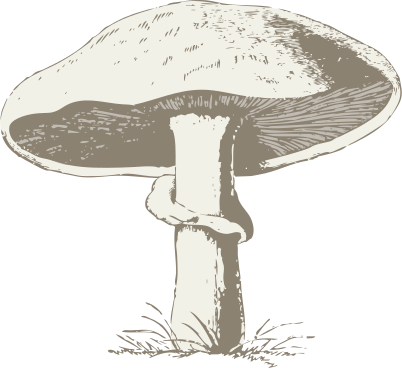
\includegraphics[width=.24\textwidth]{johnny_automatic_mushroom.pdf}
	\caption{Seta (\mushroom)}
	\label{fig:Seta}
\end{wrapfigure}
Al revisar la documentación sobre \mushroom\footnote{Ilustración obtenida en \url{https://openclipart.org/detail/900/two-mushrooms-by-johnny_automatic}} pudimos plantear mejor el problema que queríamos resolver, encontrar todas las \ARs presentes en un fichero "`pequeño"' que presenta estas características. En \href{https://archive.ics.uci.edu/ml/datasets/Mushroom}{UCI - Machine Learning Repository}\footnote{\url{https://archive.ics.uci.edu/ml/datasets/Mushroom}} describen su origen como



\selectlanguage{english}
\begin{quote}
   Mushroom records drawn from The Audubon Society Field Guide to North American Mushrooms (1981). G. H. Lincoff (Pres.), New York: Alfred A. Knopf 
\end{quote}
\selectlanguage{spanish}
\noindent Describen brevemente el contenido del fichero, indicando que se trata de setas clasificadas como comestibles o venenosas (primer valor de cada fila).
\selectlanguage{english}
\begin{quote}
\label{cita:incertidumbre-suprimida-en-mushroom}
   This data set includes descriptions of hypothetical samples corresponding to 23 species of gilled mushrooms in the Agaricus and Lepiota Family (pp. 500-525). Each species is identified as definitely edible, definitely poisonous, or of unknown edibility and not recommended. This latter class was combined with the poisonous one. The Guide clearly states that there is no simple rule for determining the edibility of a mushroom; no rule like ``leaflets three, let it be'' for Poisonous Oak and Ivy.
\end{quote}
\selectlanguage{spanish}
\noindent Y explican los valores que puede tomar cada uno de los atributos.
\selectlanguage{english}
\begin{quote}
   \footnotesize
   1. cap-shape: bell=b, conical=c, convex=x, flat=f, knobbed=k, sunken=s
   
   2. cap-surface: fibrous=f, grooves=g, scaly=y, smooth=s

   3. cap-color: brown=n, buff=b, cinnamon=c, gray=g, green=r, pink=p, purple=u, red=e, white=w, yellow=y

   4. bruises?: bruises=t, no=f

   5. odor: almond=a, anise=l, creosote=c, fishy=y, foul=f, musty=m, none=n, pungent=p, spicy=s

   6. gill-attachment: attached=a, descending=d, free=f, notched=n

   7. gill-spacing: close=c, crowded=w, distant=d

   8. gill-size: broad=b, narrow=n

   9. gill-color: black=k, brown=n, buff=b, chocolate=h, gray=g, green=r, orange=o, pink=p, purple=u, red=e, white=w, yellow=y

   10. stalk-shape: enlarging=e, tapering=t

   11. stalk-root: bulbous=b, club=c, cup=u, equal=e, rhizomorphs=z, rooted=r, missing=?

   12. stalk-surface-above-ring: fibrous=f, scaly=y, silky=k, smooth=s

   13. stalk-surface-below-ring: fibrous=f, scaly=y, silky=k, smooth=s

   14. stalk-color-above-ring: brown=n, buff=b, cinnamon=c, gray=g, orange=o, pink=p, red=e, white=w, yellow=y

   15. stalk-color-below-ring: brown=n, buff=b, cinnamon=c, gray=g, orange=o, pink=p, red=e, white=w, yellow=y

   16. veil-type: partial=p, universal=u

   17. veil-color: brown=n, orange=o, white=w, yellow=y

   18. ring-number: none=n, one=o, two=t

   19. ring-type: cobwebby=c, evanescent=e, flaring=f, large=l, none=n, pendant=p, sheathing=s, zone=z

   20. spore-print-color: black=k, brown=n, buff=b, chocolate=h, green=r, orange=o, purple=u, white=w, yellow=y

   21. population: abundant=a, clustered=c, numerous=n, scattered=s, several=v, solitary=y

   22. habitat: grasses=g, leaves=l, meadows=m, paths=p, urban=u, waste=w, woods=d
\end{quote}
\selectlanguage{spanish}

\noindent El fichero \mushroom\footnote{\url{https://archive.ics.uci.edu/ml/machine-learning-databases/mushroom/agaricus-lepiota.data}} es un fichero de texto con 8\,124 líneas, de las que muestro aquí las tres primeras:
\begin{quote}
   \footnotesize
   p,x,s,n,t,p,f,c,n,k,e,e,s,s,w,w,p,w,o,p,k,s,u
   
   e,x,s,y,t,a,f,c,b,k,e,c,s,s,w,w,p,w,o,p,n,n,g
   
   e,b,s,w,t,l,f,c,b,n,e,c,s,s,w,w,p,w,o,p,n,n,m
\end{quote}

\noindent El fichero \mushroom con el que llevo años trabajando está codificado de otro modo, conteniendo la misma información
\begin{quote}
   \footnotesize
   1 3 9 13 23 25 34 36 38 40 52 54 59 63 67 76 85 86 90 93 98 107 113
   
   2 3 9 14 23 26 34 36 39 40 52 55 59 63 67 76 85 86 90 93 99 108 114
   
   2 4 9 15 23 27 34 36 39 41 52 55 59 63 67 76 85 86 90 93 99 108 115
\end{quote}

Este modo de registrar información sobre los individuos de una población es muy habitual en todas las ciencias. Se determina qué \atributos se pueden medir, codificándolos mediante un número reducido de valores distintos, se observa a un \emph{individuo} y se mide el valor que toma en cada uno de los atributos seleccionados, obteniendo un vector de códigos.

\begin{Definition}[Individuo]
   Sean $A_i, i = 1 \ldots n$ un conjunto de atributos, siendo $n_i$ el número de valores distintos que puede tomar el atributo $A_i$. Definimos un \emph{individuo} como una $n$-túpla, un conjunto de $n$ valores obtenidos ordenadamente de los atributos $A_i$.
   $$individuo = \left(a_1, a_2\ldots a_n\right), a_i \in A_i$$
\label{def:individuo}
\end{Definition}

El propósito de recoger esta información suele ser el de \clasificacion, clasificar al \emph{individuo} en función de los valores observados en los atributos en estudio. Esta asignación se hace en función de la información que tenemos sobre esta población, generalmente un almacén \D como \mushroom, que contiene datos sobre muchos individuos de esta población correctamente clasificados.

Aunque es un problema de \Clasificacion se trata usando \arm por la forma en que se han codificado los valores expuestos para crear el fichero \mushroom. Se han utilizado números enteros consecutivos, los dos primeros para determinar la \clase (1 = \emph{venenosa}, 2 = \emph{comestible}), los siguientes para anotar el valor del atributo \texttt{cap-shape} (3 = \emph{convex}, 4 = \emph{bell}, 5 = \emph{sunken}, 6 = \emph{flat}, 7 = \emph{knobbed}, 8 = \emph{conical}), a continuación los valores del atributo \texttt{cap-surface} (9 = \emph{smooth}, 10, 11 y 12)\ldots Si encontramos \ARs fuertes entre los atributos y la \clase podemos intentar clasificar mejor a cualquier individuo de la población.







Esta estructura permite reducir notablemente la información a procesar para extraer reglas de asociación de estos ficheros, lo que convierte su estudio en una mera ejecución con \soporte mínimo nulo (si fueran más grandes podríamos averiguar antes si no están afectados por el \dilemaIR como se ha mencionado antes). Analicemos primero la estructura y veremos después una serie de características. Para entenderlo mejor analizaremos \mushroom, que es quien nos puso sobre la pista de que algo se hacía mal con este tipo de almacenes \D.

\begin{enumerate}
	\item Tiene 8\,124 filas (a las que hemos llamado \transacciones pero llamaremos \emph{registro} a partir de ahora).
	\item Cada registro tiene 23 elementos.
   \item El primer valor de cada registro es un 1 o un 2.
         
         El segundo valor es un 3, 4, 5, 6, 7 u 8.
         
         \ldots
         
         Esto nos hace pensar que cada posición del registro representa a una variable categórica. Y descubrir que los valores utilizados para representar a una variable no coinciden con los utilizados por el resto de variables, y que estos valores son consecutivos, 1\ldots119.
   % \item Si en una fila está el 1, entonces no está el 2. Esto mismo ocurre con los grupos \{3,4,5\}, \{6,7\},\ldots \{118,119\}. Esto nos hace pensar que son los valores de diferentes \atributos o \clases. Cada fila representa el valor que un individuo toma en un determinado atributo o \clase.
\end{enumerate}

%TODO: Esto va más adelante, fuera de la INTRO
En la primera lectura de \D, la que utilizamos para crear \aprioriC[1], podemos anotar la longitud de todas las \transacciones. De este modo será muy fácil comprobar si estamos trabajando con un \catalogo.

Esto sólo lo detectamos porque se han codificado los valores de cada variable categórica de modo que no haya dos iguales y sean todos consecutivos. Basta con aplicar el algoritmo mostrado en el listado~\ref{listado:comprobarCatalogo} para averiguar si \D contiene un \catalogo, una vez leído y obtenido \aprioriC[1] y $M$, el número de valores observado en todas las \transacciones.

\lstinputlisting[label=listado:comprobarCatalogo,
                 caption={Comprobación sobre \catalogos},
                 float=htb,
                 basicstyle=\footnotesize]
                 {./contenido/clasificacion/codigo/algComprobarCatalogo}


   % \item No hay dos registros iguales. Esto nos hace pensar que se trata de un \textbf{\catalogo}, no de una \textbf{muestra}. Aunque en ambos casos la reducción de información a procesar que podemos es la misma (en la muestra\ldots) la información que obtendremos no es la misma, lo que se explica en la sección~\ref{sec:3-3-CatalogoVsMuestra}.

Un \catalogo tiene una estructura muy rígida. Si hay valores missing se puede añadir un valor al atributo en cuestión indicando esa circunstancia, o no utilizar la información del atributo en cuestión o incluso hacer una estimación del valor si se puede justificar.

En un \catalogo todos los registros contienen $n$ datos, y si forma parte de una tarea de \clasificacion uno o varios de esos datos representan una \clase, generalmente el "`\atributo"' cuyo valor queremos determinar a partir de la observación de los valores del resto de \atributos.

\begin{Definition}[Registro]
   Sean $A_i, i = 1 \ldots n$ un conjunto de atributos, siendo $n_i$ el número de valores distintos que puede tomar el atributo $A_i$. Definimos un registro como una $n$-túpla, un conjunto de $n$ valores obtenidos ordenadamente de los atributos $A_i$.
   $$registro = \left(item_1, item_2\ldots item_n\right), item_i \in A_i$$
\label{def:registro}
\end{Definition}

\begin{Definition}[\Catalogo] Un \catalogo es un conjunto de $N$ registros diferentes.
   $$\catalogo = \left\{registro_i, i = 1\ldots N\ | \ registro_i \neq registro_j \forall i \neq j\right\}$$
\label{def:catalogo}
\end{Definition}
% \borrar{Buscar una definición mejor, en \clasificacion}


El número de combinaciones entre todos los valores de los atributos en estudio es muy grande, sin embargo cuando se está haciendo un estudio real no se obtendrán todas las combinaciones posibles. En un \catalogo sólo están las combinaciones que interesa estudiar, básicamente aquellas que sí se dan en la población en estudio. Es una selección de los registros que se podrían formar con todas las combinaciones de valores proporcionada por los atributos en estudio.

La esencia de un \catalogo es que no tiene registros repetidos. Si tomamos una muestra de una población midiendo en cada individuo todos los valores de los atributos del estudio es muy probable que en la muestra existan registros repetidos. Las muestras de este tipo se verán a fondo en la sección~\ref{sec:clasificacion:catalogo:muestras}, es importante estudiar sus diferencias con los \catalogos pues contienen información sensiblemente diferente.

Un \catalogo puede cambiarse fácilmente, basta con cambiar el número de valores que puede tomar una de las variables en estudio para que cambie por completo el \catalogo. Una muestra no puede cambiarse, se obtiene de la realidad, se diseña previamente y si se quiere añadir a otra muestra en que se han utilizado otros valores debería rehacerse\ldots


Si aprovechamos esta información podemos reducir notablemente los ítems a procesar sin perder la información que contiene el \catalogo (o muestra) completo\ldots

% \borrar{Aquí viene el ejemplo de Interacción'12, he de buscar cómo escribir código.}







%\subsection{\Catalogo comprimido}
%\label{sec:3-1-1-CatalogoComprimido}
%\input{./3-ARMCatalogos/3_1_Catalogos/3_1_1_CatalogoComprimido}
%
%
%
%
%
%
%
%\subsection{Lectura de \catalogo comprimido}
%\label{sec:3-1-2-LecturaDeCatalogoComprimido}
%\input{./3-ARMCatalogos/3_1_Catalogos/3_1_2_LecturaDeCatalogoComprimido}
%
%
%










Los catálogos son colecciones de registros preparadas para resolver informáticamente un problema de clasificación. Y muchos investigadores de esta especialidad publican sus datos para que otros investigadores puedan hacer pruebas con las mismas condiciones de partida: una colección de datos con ciertas características. En UCI, KEEL, LUCS\ldots encontraremos muchos catálogos entre los datasets que publican para resolver problemas de clasificación.\marginpar{\footnotesize Acabo de descubrir LUCS, que discretiza las colecciones de UCI y me ofrece 97 valores distintos en adult, frente a los 27\,245 que tiene el de UCI, he de analizarlo con mi código y EXPLICAR MEJOR LAS CONSECUENCIAS DE APLICAR ANTES O DESPUÉS MI MÉTODO O LA AGRUPACIÓN DE VALORES EN ATRIBUTOS NUMÉRICOS ya que se obtendrán reglas y catálogos completos bastante diferentes, esto da para otro artículo y más si tengo en cuenta que tiene datos missing por lo que puedo obtener catálogos completos usando menos atributos con más registros o catálogos completos usando sólo los atributos registrados en cada registro (a no ser que el análisis nos diga que cierto atributo no aporta información\ldots.}

Cuando no sabíamos que esos ficheros contenían catálogos intentábamos aplicar bien conocidos algoritmos de ARM pero no podíamos extraer información que contienen los datos porque se desbordaba la RAM del equipo en que se está aplicando el algoritmo y se abortaba el proceso tras horas de cálculos que finalmente no obteníamos. Esto nos sorprendía porque el primer catálogo que intentamos analizar con Apriori sólo tiene 5\,644 registros de 23 datos, no son números excesivos para un problema de Minería de Datos analizado con un ordenador de escritorio con cierta potencia y capacidad de RAM. Eso nos llevó a descubrir cómo se creó el catálogo a través de \url{UCI/mushroom}\ldots

Los catálogos caracterizan un problema de clasificación concreto. Si queremos plantear otro problema de clasificación, bien etiquetando a los mismos individuos en otras \clases o bien utilizando atributos diferentes no podemos utilizar directamente cualquier catálogo que tengamos sobre la misma población. Si los dos problemas usaran los mismos atributos pero diferentes \clases y las \clases en estudio son independientes no servirá de nada la información que tengamos sobre los catálogos completos del primer problema de clasificación si no sabemos analizar qué información puede ser relevante y cuál no, de hecho la información menos relevante en esta situación es la distribución de las \clases en cada uno de los problemas de clasificación por lo que debemos huir de interpretaciones erróneas utilizando estos datos para estimar soportes o confianzas poblacionales.

De un catálogo se puede extraer información válida para otro problema de clasificación que utilice los mismos atributos ya que si en la muestra en que se basa el catálogo no presenta cierta relación entre los valores de los atributos YA SABEMOS QUE NO APARECERÁ ESA RELACIÓN AUNQUE CAMBIEMOS DE CLASES (siempre que el catálogo sea válido, aún tengo que hacer muchas definiciones sobre muestra, población, distribución de \clases, problema de \clasificacion, \atributos, \clases, \catalogos, catálogos completos, validez de un catálogo\ldots).

Aunque la \ARM busca cualquier relación entre cualquier par (o $k$-itemset) de valores de \D, el objetivo del problema de \clasificacion es siempre el mismo, etiquetar cada \registro con una \clase basándose en la información disponible sobre otros \registros con valores idénticos en sus \atributos.





\subsection{Muestras}
\label{sec:clasificacion:catalogo:muestras}
La importancia que se da en todos los estudios de \ARM al \soporte de una \ar se justifica cuando se trabaja con muestras, que no contienen la misma información que un \catalogo. Para obtener una muestra en un problema de \clasificacion se han de seleccionar individuos de una población, medir en cada uno de ellos el valor que toma cada uno de los \atributos en estudio y averiguar la \clase a la que pertenece. Al guardar todos los \registros obtenidos de este modo es posible que existan \registros repetidos, lo que aporta información sobre la distribución de la población en estudio con un elevado coste sobre los \catalogos ya que en estos no deberíamos repetir el registro si no añadir un número entero indicando el número de veces que aparece el \registro en la muestra.






\section{\CC}
\label{sec:clasificacion:catalogo-completo}
% !TEX root = ../../Lazcorreta.Tesis.tex
\ABIERTO
Al seguir trabajando con \mushroom encontramos otra versión del mismo dataset en KEEL

http://sci2s.ugr.es/keel/dataset.php?cod=178


\borrar{Necesito definir antes conjuntoDeValoresDeAtributos, quizá en otra sección.}
\begin{Definition}[\CC] Un \CC es un \catalogo sin incertidumbre.
   $$\CC = \left\{registro_i, i = 1\ldots N\ | \ registro_i \neq registro_j \forall i \neq j\right\},  conjuntoValoresAtributos son todos diferentes$$
\label{def:catalogo}
\end{Definition}






\subsection{Colecciones de \CCs}
\label{sec:clasificacion:catalogo-comprimido:colecciones}
%\input{contenido/clasificacion/catalogo-comprimido/colecciones}

Todos los \CCs pueden tener un \CC maximal y diversos \CCs de menores dimensiones. Volviendo al origen de esta investigación, disponemos de un dataset\ldots





%TODO: Añadir \missing al índice alfabético
\section{Datos missing}
\label{sec:clasificacion:datos-missing}
% !TEX root = ../../Lazcorreta.Tesis.tex
\ABIERTO
%TODO: Incluir "datos missing" en indice-alfabetico
\mushroom contiene 8\,124 registros en su dataset original de la UCI, sin embargo en el fichero KEEL con el que hemos trabajado desde la sección~\ref{sec:catalogo:catalog} contiene sólo 5\,644 registros porque se han eliminado los \registros con datos missing que contenía el fichero original. Para diferenciar ambos \datasets llamaremos \texttt{mushroom-original} al \dataset de la UCI y \texttt{mushroom-reducido} al que no contiene datos missing.

En un problema de \dm los datos missing no deberían ser considerados. El objetivo de esta disciplina es la obtención de información (previamente desconocida) a partir de los datos. Un dato missing no aporta información como dato, podría ser interpretado en muchos experimentos el hecho de no conocer ese dato pero el dato en sí no lo conocemos y, por lo tanto, no podemos usarlo. Se podrían estimar a partir de los datos que sí conocemos pero si no hay una justificación suficientemente poderosa no deberíamos "`inventar"' ningún valor cuando queremos obtener la información que contienen los datos que realmente conocemos. La \dm se aplica a los datos conocidos o estimados pero en este momento sólo tenemos datos missing sin interpretar por lo que no nos pueden dar ningún tipo de información.

Cualquier \ar que incluya el ítem \texttt{stalk-root=?} en su antecedente debe ser ignorada ya que su interpretación sería "`\emph{Si no sé qué valor tiene stalk-root entonces\ldots}"'.

%TODO: He cambiado la referencia a catalogo-comprimido por catalogo-completo. Comprobar que es correcto.
En un registro, la ausencia de un dato provocará tener un valor menos, lo que traducido a transacciones se convierte en una transacción de distinto tamaño que el resto de registros. Esto sería un problema para tratarlo como se ha propuesto en la sección~\ref{sec:clasificacion:catalogo-completo} ya que el fichero \D no será considerado \catalogo por no tener todos sus registros el mismo tamaño. Una solución consiste en considerar el valor missing de un atributo como un valor distinto al resto de los que realmente contiene, en el caso de \mushroom se denota con \texttt{?}, al convertirlo en fichero \D se codificará ese valor como un valor distinto del atributo al que pertenezca y la única consecuencia es, aparentemente, que tenemos un ítem diferente más.

Los datos missing son difíciles de interpretar correctamente ya que para convertir los ficheros en formato adecuado para ARM se utiliza un código binario para indicar esta situación, i.e., si un registro no contiene información sobre un atributo se crea la categoría ficticia "`dato desconocido"' en dicho atributo y se le asigna esa categoría, así podemos aplicar con cierta normalidad las técnicas de ARM, aunque la interpretación de las reglas que se pueden obtener es confusa:

\begin{quote}
Si no conocemos el valor del atributo $\A_i$ podemos deducir que\ldots
\end{quote}

Eliminar los registros con datos missing parece una estrategia correcta para no tener que gestionar estas \ars. Sin embargo perdemos información sobre 2\,480 registros, sin saber si la información que perdemos es relevante o no lo es.

Si analizamos el fichero \mushroom observaremos que sólo un atributo contiene datos missing, \texttt{stalk-root}, y ya hemos visto en la sección~\ref{sec:clasificacion:catalogo-completo} que este atributo es prescindible, al menos en el dataset reducido de KEEL. Con lo que ahora sabemos sobre \catalogos podemos diseñar otra estrategia, eliminar el atributo \texttt{stalk-root} del dataset original y comprobar si esos 2\,480 registros ignorados por la estrategia utilizada contienen información que habíamos perdido irremediablemente.

En \urlConNotaAlPie{http://sci2s.ugr.es/keel/dataset.php?cod=178}{KEEL - Mushroom} proporcionan dos ficheros \mushroom:
\begin{itemize}
  \item por defecto el que han elaborado con su formato tras eliminar los registros con datos missing, con 5\,644 registros\footnote{\scriptsize\url{http://sci2s.ugr.es/keel/dataset/data/classification/mushroom.zip}},
  \item si lo buscamos nos ofrecen el dataset original en formato KEEL, con 8\,124 registros\footnote{\scriptsize\url{http://sci2s.ugr.es/keel/dataset/data/missing/mushroom.zip}}.
\end{itemize}
Al analizar ambos ficheros se obtienen los siguientes resultados:
\begin{enumerate}
  \item \texttt{mushroom-original} contiene un \sCC de 8\,124 \registros, con un atributo que contiene datos missing, \texttt{stalk-root}, que es prescindible y no aumenta el tamaño del \catalogo.
  \item \texttt{mushroom-reducido} contiene un \sCC de 5\,644 \registros, \texttt{stalk-root} es prescindible y no aumenta el tamaño del \catalogo.
\end{enumerate}
Luego tenemos dos análisis sobre dos \datasets que ofrecen datos similares pero deben contener diferente información. Analizar sus similitudes y diferencias nos dará más información que la que obteníamos con el primer fichero KEEL. Destaquemos que:

\begin{enumerate}
  \item Ambos ficheros son \sCCs. Todos sus \registros son distintos y no contienen incertidumbre.
  \item Si eliminamos en cualquiera de ellos el atributo \texttt{stalk-root} no se reduce el \catalogo ni se pierde información. No sabemos si \texttt{mushroom-reducido} seguirá siendo un \sCC.
\end{enumerate}
Si no sobran los 2\,480 registros de más que tiene el \CC original deberían de aportar algo de información que no está presente en el \catalogo reducido. Esto lo sabremos tras eliminar su atributo \texttt{stalk-root} y comprobar si genera incertidumbre\borrar{Explicarlo con ecuaciones}.
\begin{itemize}
  \item Si no la genera es por\ldots
  \item Si la genera es por\ldots
\end{itemize}



Si eliminamos \texttt{stalk-root} de ambos ficheros obtendremos dos \sCCs distintos, el primero con todos los registros-tipo del segundo y además 2\,480 registros-tipo que no están en el segundo. Es evidente que el primero tiene información más precisa sobre el problema de \clasificacion que estamos analizando. Pero la información extra que contiene no es sobre el atributo \texttt{stalk-root}, ni tan siquiera se utiliza este atributo para obtener esa información, sólo depende de las co-ocurrencias entre valores del resto de atributos. Si eliminamos el atributo \texttt{stalk-root} de ambos ficheros obtendremos dos nuevos \sCCs, esta vez sin datos missing, ambos orientados al mismo problema de \clasificacion y sin ninguna discrepancia entre ellos (de hecho el reducido es una partición del original). Si pudiéramos utilizar cualquiera de ellos en nuestro próximo clasificador está claro que deberíamos usar el \sCC que ese obtiene eliminando el atributo \texttt{stalk-root} al dataset original.

El \sCC mayor contiene al menor pero el menor se ha obtenido a partir de la información proporcionada por otro atributo (que ahora ya no está). Ambos contienen algo de información distinta para el mismo problema de \clasificacion. En el menor hay más $ARN_2$, que desaparecen al añadir nuevos registros-tipo para formar el mayor, es lo que podría ocurrir si seguimos tomando muestras y aparecen nuevos registros-tipo que no presenten incertidumbre, el \sCC va mejorando y nos informa que los datos que conocemos garantizan una buena clasificación (no es necesario medir otro atributo porque no tenemos incertidumbre y cada vez sabemos más sobre los registros-tipo de este problema de clasificación).







No todos los \catalogos con datos missing tendrán las mismas características que \mushroom, pero sí se puede dar en muchos estudios que sigamos añadiendo registros a un dataset pero sin incluir el valor de uno de sus atributos, si el resto de atributos es suficiente para clasificar correctamente al individuo tendremos una situación similar a la analizada en esta sección. Si estamos trabajando con un \sCC completo y válido es muy posible que no necesitemos nunca más medir el valor de ese atributo, pero no deberíamos borrarlo del dataset original porque alguna vez podría aparecer algo de incertidumbre en el \catalogo y sería útil poder añadir toda la información que ya se recogió en su día sobre cualquier otro atributo medible en los individuos en estudio.






\section{Publicaciones}
\label{sec:clasificacion:publicaciones}
% !TEX root = ../../Lazcorreta.Tesis.tex
En Interacción'12 comenzamos a publicar nuestros resultados sobre las colecciones de \transacciones estructuradas mediante \catalogos. Los mayores avances los hemos obtenido este último año y estamos en un proceso actual de publicación de resultados en diversas revistas y un nuevo congreso internacional.





%\cite{Lazcorreta:Botella:FCaballero:EfficientAnalysisOfTransactionsWebRecommendations:2012}
\subsection*{Efficient analysis of transactions to improve web recommendations, 2012}

\begin{quote}
  Lazcorreta Puigmartí, E., Botella Beviá, F. y Fernández-Caballero, A. Efficient analysis of transactions to improve web recommendations. {\em Actas del XIII Congreso Internacional de Interacción Persona-Ordenador}, ACM International Conference Proceeding Series, 2012. \leePDF{bib/nuestros/LazcorretaBotellaFCaballero-EfficientAnalysisOfTransactionsWebRecommendations-2012.pdf}
\leePDF{bib/nuestros/LazcorretaBotellaFCaballero-AnalisisEficienteDeTransacciones-2012-Presentacion.pdf}
\scopus{http://www.scopus.com/inward/record.url?eid=2-s2.0-84869053054&partnerID=40&md5=ded243c196907c1e6eec90cd9624ab3d}
\descargaRevisado{https://www.researchgate.net/publication/266652926_Efficient_analysis_of_transactions_to_improve_Web_Recommendations}
\descargaRevisado{https://www.deepdyve.com/lp/association-for-computing-machinery/efficient-analysis-of-transactions-to-improve-web-recommendations-mBuBBNIv7c}
\github{https://github.com/EnriqueLazcorreta/tesis-0/blob/master/bib/nuestros/LazcorretaBotellaFCaballero_EfficientAnalysisOfTransactionsWebRecommendations_2012.pdf}
\github{https://github.com/EnriqueLazcorreta/tesis-0/blob/master/bib/nuestros/LazcorretaBotellaFCaballero_AnalisisEficienteDeTransacciones_12_Presentacion.pdf}
\end{quote}

\begin{quotation}
	\noindent\textbf{Resumen}

	\nopagebreak When we deal with big repositories to extract relevant information in a short period of time, pattern extraction using data mining can be employed. One of the most used patterns employed are Association Rules, which can measure item co-occurrence inside large set of transactions. We have discovered a certain type of transactions that can be employed more efficiently that have been used until today. In this work we have applied a new methodology to this type of transactions, and thus we have obtained execution times much faster and more information than that obtained with classical algorithms of Association Rule Mining. In this way we are trying to improve the response time of a recommendation web system in order to offer better responses to our users in less time. Copyright 2012 ACM.
\end{quotation}








\subsection{[...]}
En la actualidad estamos completando la redacción de un artículo sobre esta fase de nuestra investigación, que será enviada en breve para su revisión y posible publicación en revista. En él se exponen la teoría y experimentos que forman la sección~\ref{sec:clasificacion:catalogo-completo}.




\subsection{[...]}
La Interacción Persona-Ordenador es una disciplina en la que se analizan muchos catálogos por lo que presentaremos nuestra aportación a esta rama de la ciencia en el Congreso Internacional Interacción'16, que se celebrará en septiembre de 2016 en Salamanca.
